
\subsection{A--A$_3$Si--A$_5$SiB$_2$ Eutectics}

Mo$_5$SiB$_2$, a T2 phase (Figure: \ref{T2structure}), is an extremely creep resistant phase at high temperature ~\cite{rawn01}. Incorporating it can allow for improvements in creep properties. Unfortunately, chromium additions would destabilise the T2 phase. This phase forms via a peritectic reaction, and would require further alloying additions to either tease it into a eutectic reaction, or to counter Cr's T2 phase de-stabilization. 
%
\begin{figure}[H]
\begin{center}
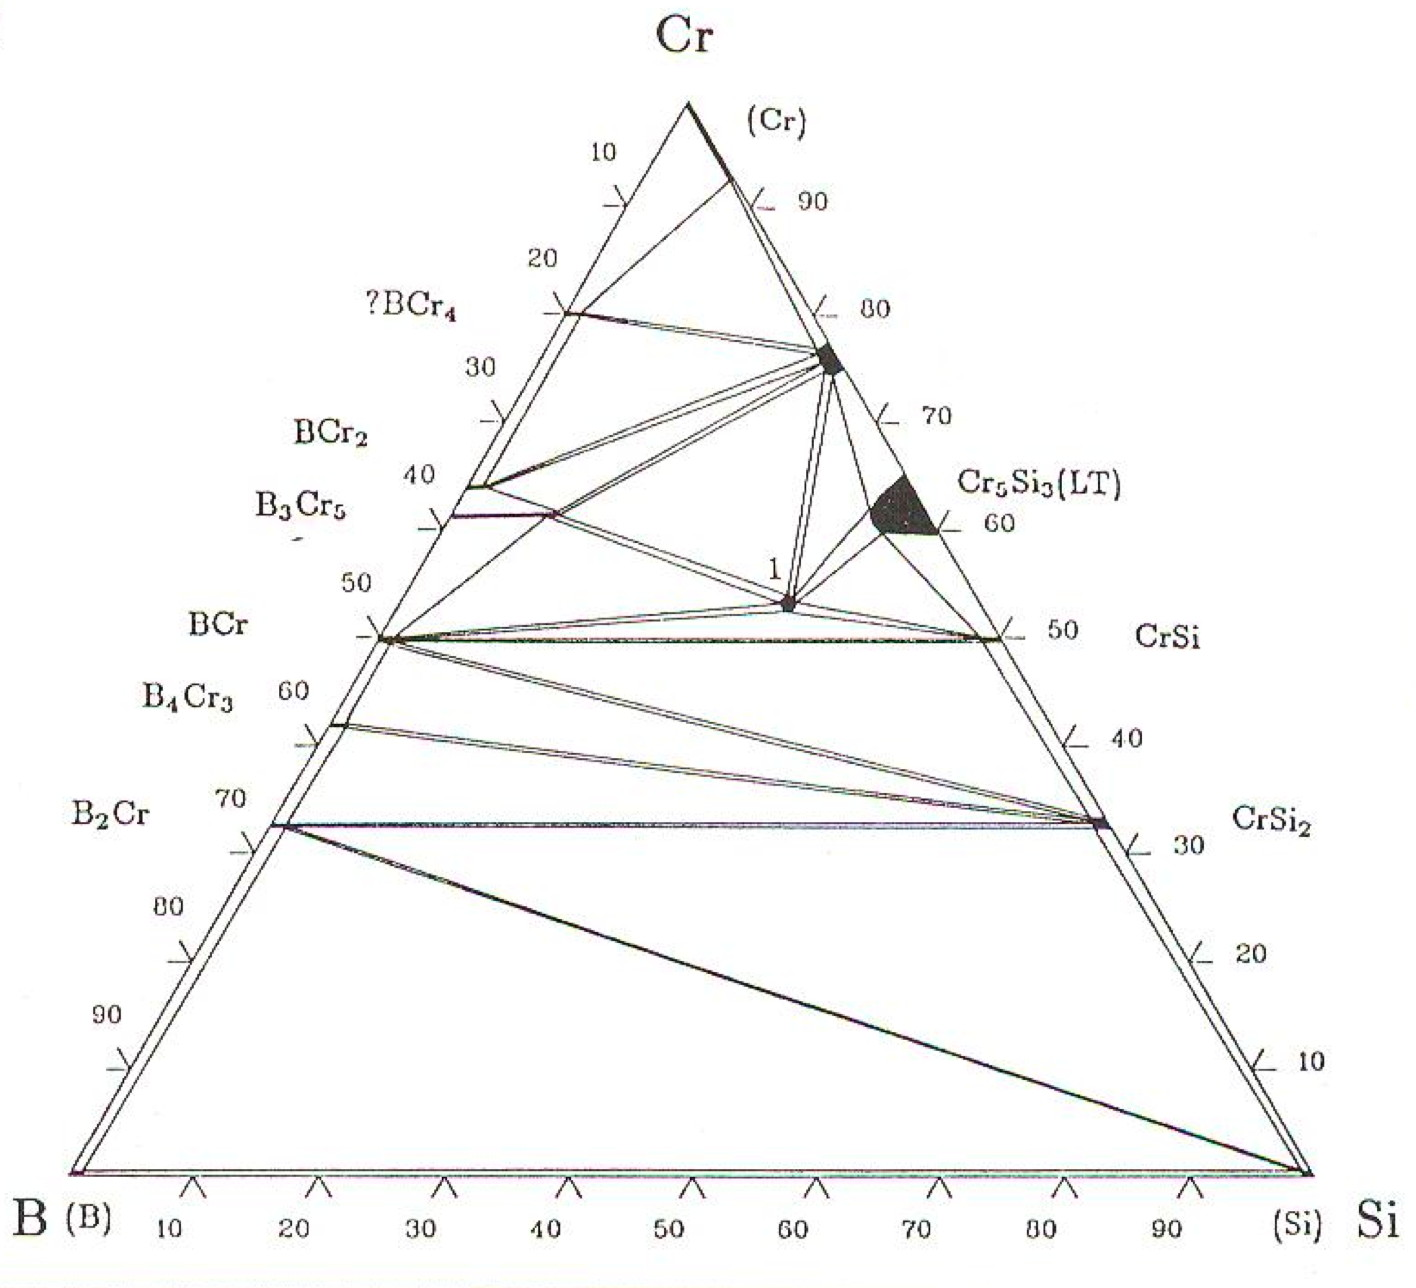
\includegraphics{CrSiB}
\caption{Ternary phase diagram of Cr--Si--B.}\label{fig:CrSiB}
\end{center}
\end{figure}
%
\begin{figure}[H]
\begin{center}
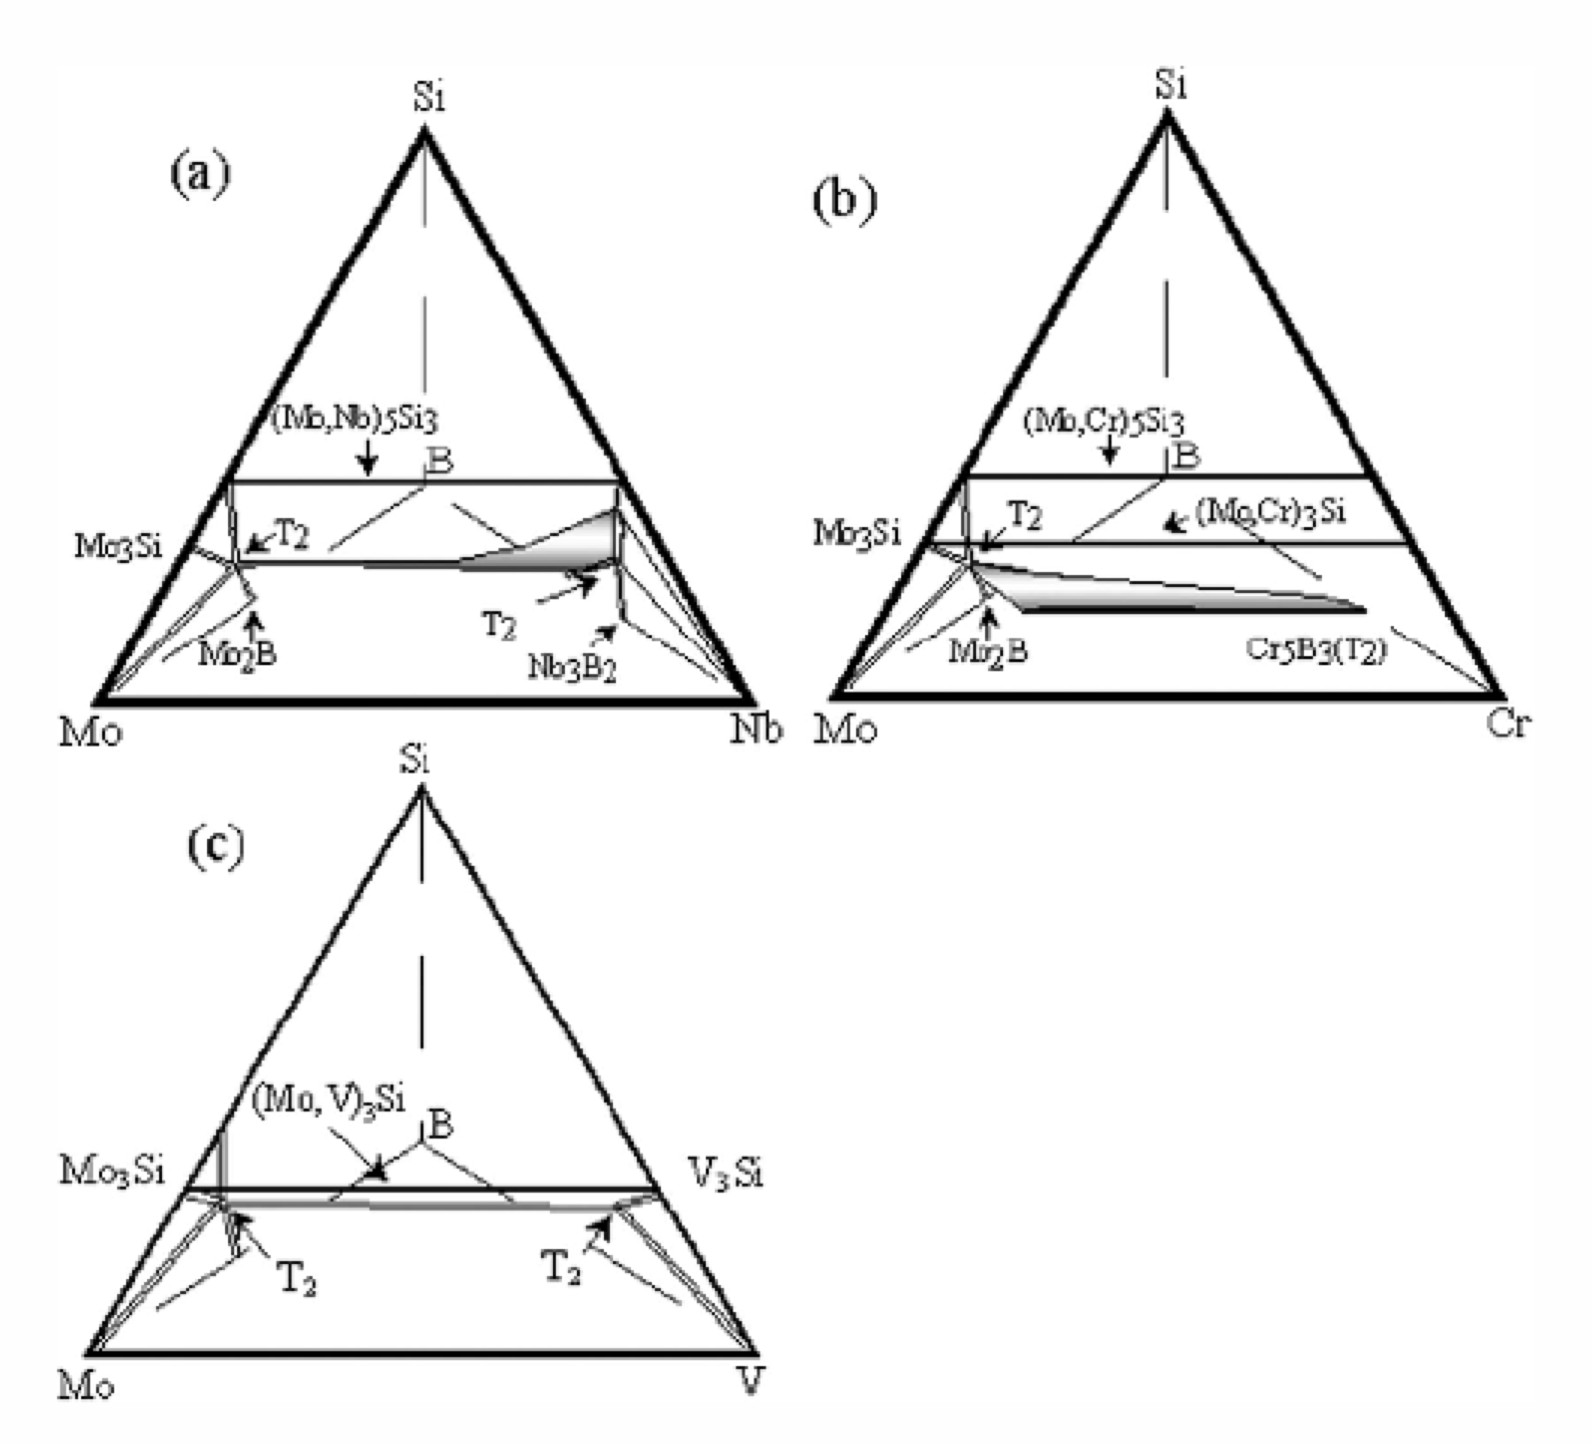
\includegraphics{T2_alloying}
\caption{Schematic illustration of observed solubility for selected transition metal (TM) substitutions in both the bcc and the T2 phase in the quaternary Mo--TM--Si--B. (sakidja05)}\label{fig:T2_alloying}
\end{center}
\end{figure}
%
There is no ternary phase diagram available for the V--Si--B system (ASM) except for the schematic seen in Sakidja and Perepezko ~\cite{sakidja05}. The analogous V$_5$SiB$_2$ has been reported. An approach to incorporate T2 into our eutectic structure would be to ascertain if a A--A$_3$Si--A$_5$SiB$_2$ eutectic occurs in this system. The threshold of chromium concentration at which the A$_5$SiB$_2$ phase becomes destabilised in the (Cr,V)--(Cr,V)$_3$Si--(Cr,V)$_5$SiB$_2$ ternary eutectic will then be assessed. If this proves successful, the eutectic will be extended to (Cr, Mo,V)--(Cr, Mo,V)$_3$Si--(Cr, Mo,V)$_5$SiB$_2$. Mo additions can further stabilise the T2 phase. Rawn reports that B substitutes for Si to a limited extent, which suggests that the composition of T2 is not necessarily stiochiometric. During extension of the ternary V--Si--B system to include more elements, this B--Si ratio may change.

\section{Experimental Method}
\subsection{Silicides}

The (Cr,V)--(Cr,V)$_3$Si tie-line will be determined by arc-melting a set of five ingots of estimated compositions. As these alloys are expected to be brittle and hard at room temperature, sample machining will be done by electro-spark machining if cutting with a diamond saw proves unsuccessful. They will prepared for optical examination by implanting in Bakelite� and polished to a .05\micro\meter\ finish. They will then be etched with Murakami solution, as detailed by Bei et al.. The volume fraction of pro-eutectic phases in these ingots will be gauged by examining their microstructure using an optical microscope. Their compositions will be analysed using EDS. Chromium is more volatile than the other elements, and chromium losses are expected during manufacture. Compositions will be adjusted to eliminate pro-eutectic phases, and this process will be iterated till optimised eutectic microstructures are obtained. 

** nominal compositions of (Cr,V)--(Cr,V)$_3$Si arc-melt alloys

Isothermal oxidation at 800\celsius\ and 1150\celsius\ for 100 hours will be conducted on the tie-line eutectics as an initial investigation of the characters of oxides formed. Cyclic oxidation may be performed if time permits. Once successful, the same process will be iterated for subsequent molybdenum substitutions to the (Cr,V)--(Cr,V)$_3$Si eutectics that have been found to be oxidation resistant. 
** nominal compositions of (Cr,V,Mo)--(Cr,V,Mo)$_3$Si arc-melt alloysPolycrystalline lamellar Cr--Cr$_3$Si will be cast using the department�s radio frequency (RF) furnace. It does not have the capability to cast the V--V$_3$Si eutectic as its maximum casting temperature is 1800\celsius, 70\celsius below the eutectic's melting point. Other equipment will have to be sought. One alternative is a 4-mirror image furnace with a temperature capability of 2800\celsius. This is available at the Physics Department at the University of Warwick. Lamellar Cr--Cr$_3$Si and V--V$_3$Si can be cast there, as this furnace has a maximum casting rate of 18mm/h. Attainment of single-crystal material and elimination of pro-eutectic phases will require a few iterations of castings. Once optimised polycrystal or single-crystal microstructures are obtained, creep samples will be electro-spark machined, and either compression or tensile creep will be performed at 1150\celsius\ and 1200\celsius. This creep data will be compared to available data on a representative commercially available nickel-base superalloy CMSX-4. Other equipment will have to be sought to cast cellular Cr--Cr$_3$Si and V--V$_3$Si. If this is successful, creep data will be collected on these alloys. A method will have to be found to manufacture TEM specimens. TEM will be performed on the as-crept samples to look at dislocation behaviour.

\subsection{Boro Silicides}
The existence of the ternary eutectic of V--V$_3$Si--V$_5$SiB$_2$ will be determined. A series of ingots with varying concentrations of boron added to the V--� V$_3$Si eutectic will be made by arc-melting. Microstructural and compositional analysis will be carried out using optical microscopy, SEM and EDS. ** nominal compositions of V--V$_3$Si-- V$_5$SiB$_2$ arc-melt alloys. If the ternary eutectic is found, isothermal oxidation will be performed. We will attempt to cast it using the 4-mirror image furnace and determine its creep properties. Chromium substitutions of vanadium will be made to investigate the extent of ternary eutectic destabilisation.** nominal compositions of (Cr,V)--(Cr,V)$_3$Si--(Cr,V)$_5$SiB$_2$ arc-melt alloys

\section{Results}
Arc-melt ingots have been made of Cr--Cr$_3$Si and V--V$_3$Si. The vacuum system of the arc-melt facilities in the department may not be good enough, as the Cr � Cr$_3$Si ingots seem to suffer from nitrogen embrittlement. There is a National Laboratory at the University of Birmingham that has arc-melt and skull-ingot facilities. Some samples will be made in Birmingham to see if purer and more homogeneous samples can be achieved.2 castings of the Cr � Cr$_3$Si eutectic were done using the radio frequency furnace in Cambridge. The first cast was allowed to equilibriate at 1740\celsius, 35\celsius\ above eutectic melting point, for 1 hour, before being withdrawn at 20 mm/hr. When the alumina crucible was broken open after the cast, the feed arc-melt ingot was found to have only partially melted. The hold time was possibly not long enough for the ingot to melt, and the hot zone could be smaller than the feed ingot, and only the portion within the hot zone melted. The second cast was equilibriated at 1780\celsius\ for an hour. A better melt was achieved before this cast. Peering down the opening of the cylindrical crucible, a meniscus was seen. Under the circumstances, that was the best measure of the degree of melting of the feed ingot. This ingot was also solidified at 20 mm/hr. Due to reaction between the alumina crucible and cast ingot, the ingot had to be broken out of the crucible. This ingot seemed to have been cast well. Microstructural and compositional analysis have not been performed on the ingots yet, due to difficulties in getting the ingot cut. The electro-spark machining equipment at the department were unsuccessfully employed. The samples had to be out-sourced for machining.**photos of cast ingotsA cast was performed using the 4-mirror furnace at the Physics Department of the University of Warwick. The casting rate was at the furnace�s maximum drawing rate of 18mm/h. Despite using an ingot that had undergone several arc-melts, inhomogenities still persisted, and the melt could not be sustained as the melting temperature of the feed ingot fluctuated too much. Due to the finicky nature of the cast, the melt broke three times. Melt contact was re-established each time, but this meant that the grains were discontinuous, and there is not enough uninterrupted length to machine out a creep specimen.photo of seed and feed crystals used in cast
%
\begin{figure}[H]
\begin{center}
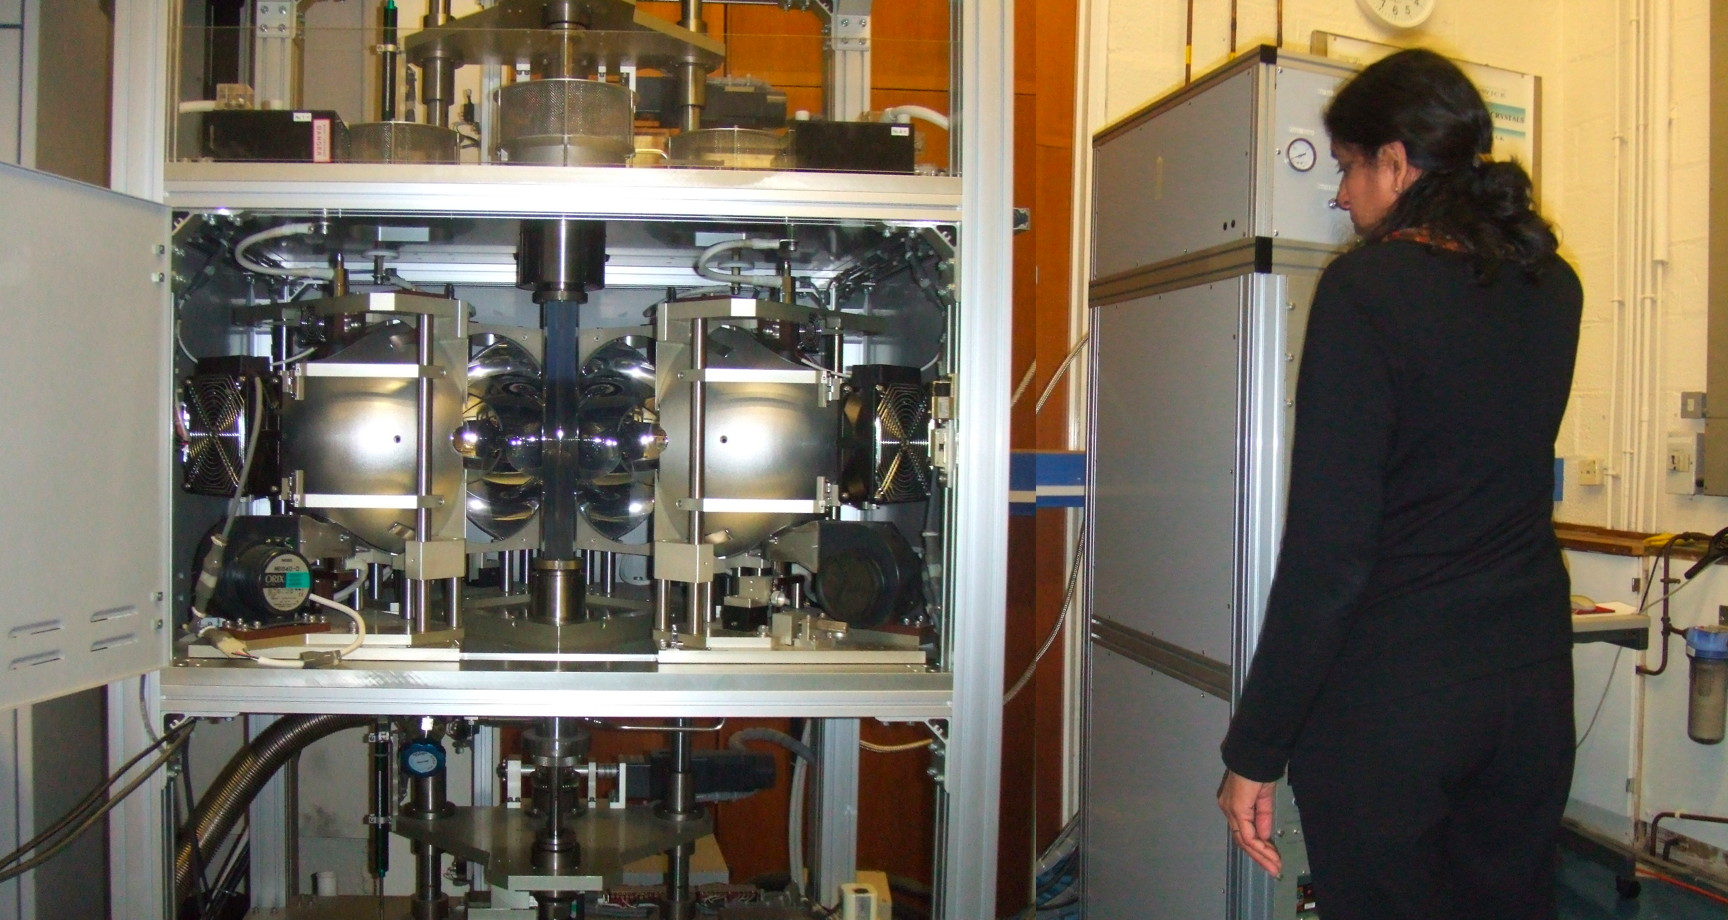
\includegraphics{MirrorFurnace}
\caption{Photo of the 4-mirror furnace at the University of Warwick.}\label{fig:MirrorFurnace}
\end{center}
\end{figure}
%
\begin{figure}[H]
\begin{center}
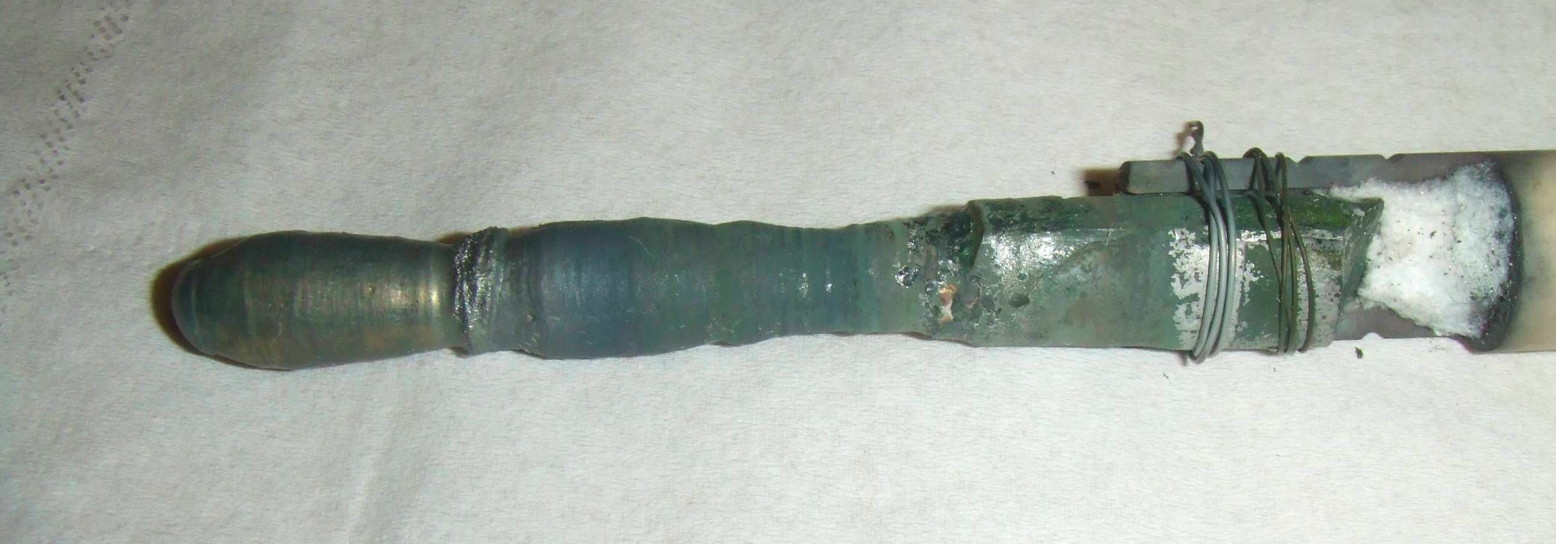
\includegraphics{FirstCast}
\caption{Photo of our 1st directionally solidified Cr-Cr$_3$Si ingot.}\label{fig:FirstCast}
\end{center}
\end{figure}
%
At this casting rate, a lamellar microstructure should be seen. However, there is too much dendritic chromium solid-solution pro-eutectic in the microstructure disrupting lamellae formation. Only about 2\% of the area fraction of the transverse section was lamellar. 	 
%
\begin{figure}[H]
\begin{center}
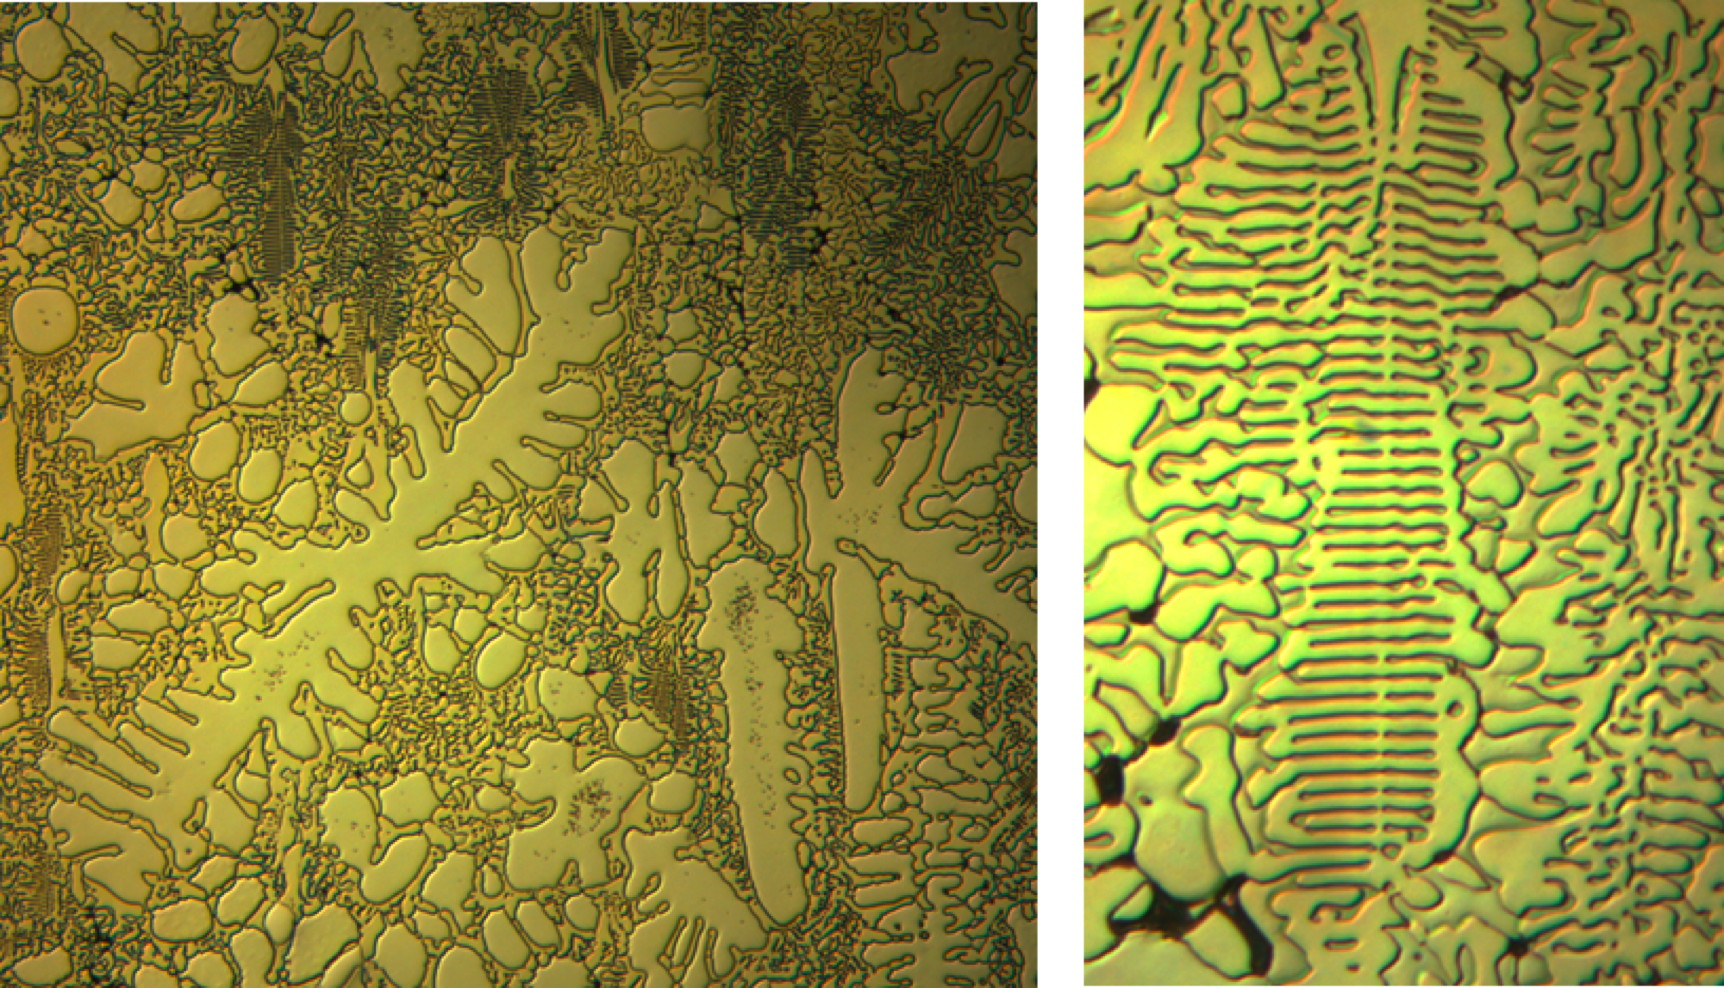
\includegraphics{FirstCast_trans}
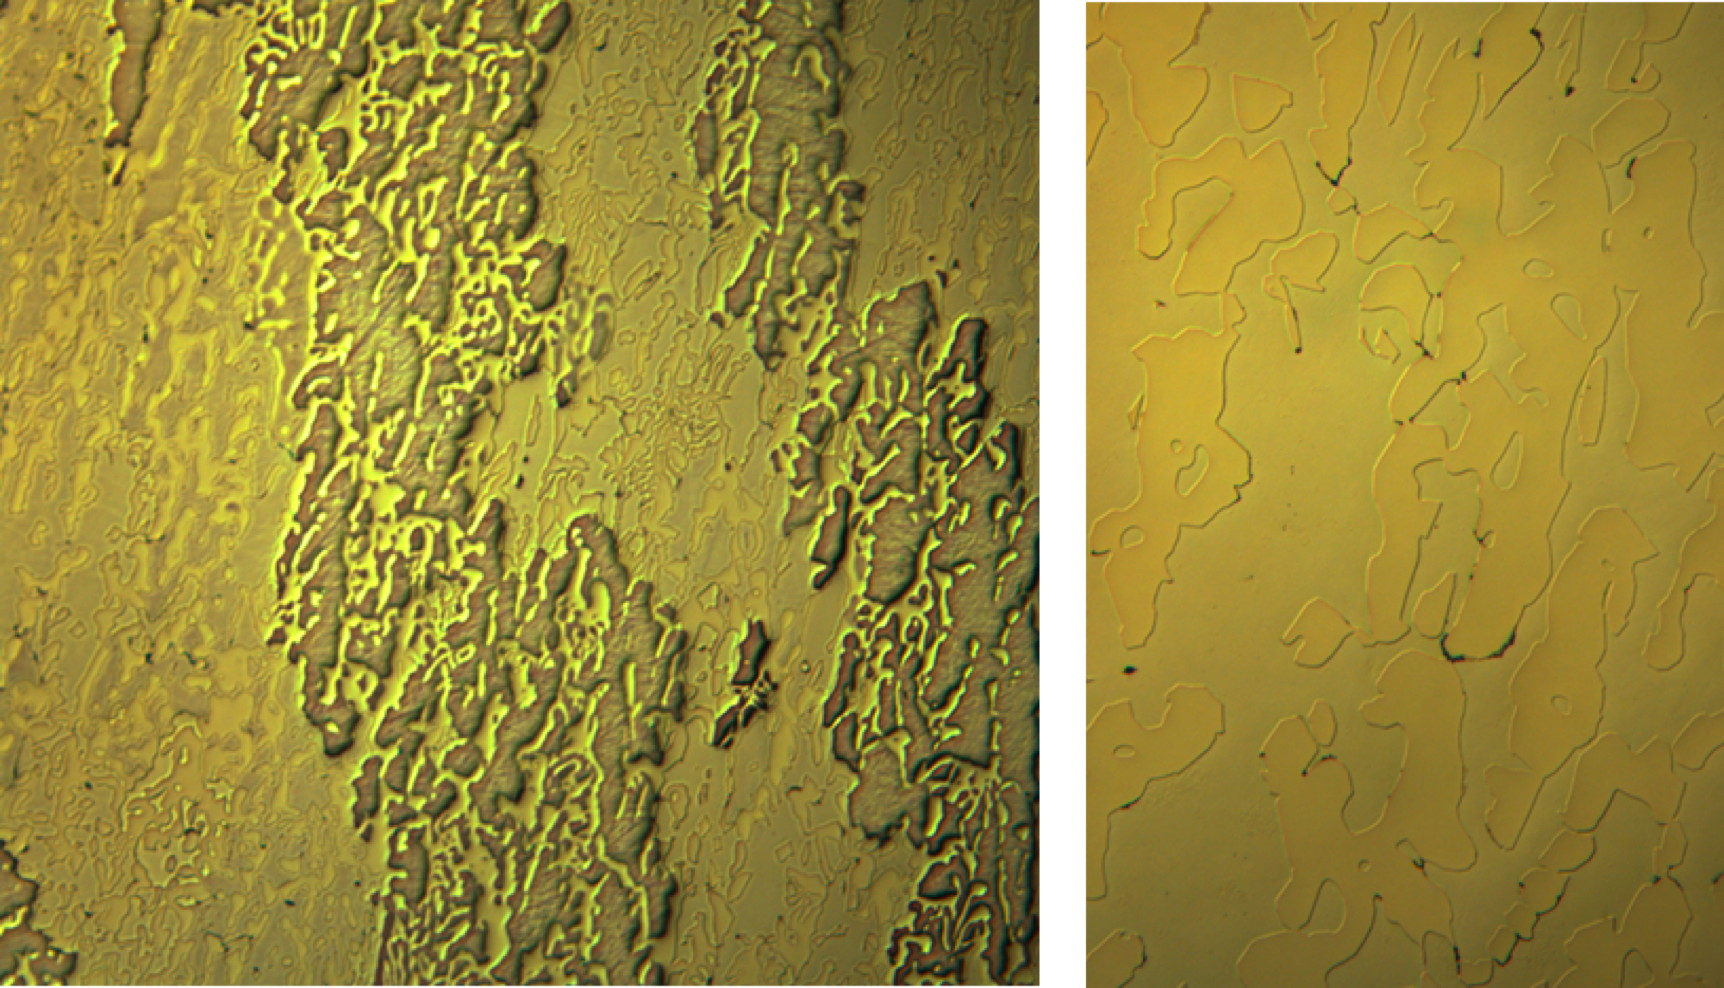
\includegraphics{FirstCast_long}
\caption{Microstructures obtained during the 1st cast using the 4-mirror furnace. Longitundinal sections of seed crystal, cast with arc-melt seed ingot, cast from directionally-cast seed crystal, transverse section of cast from directionally-cast seed crystal.}
\label{fig:FirstCast_micros}
\end{center}
\end{figure}
%

Energy Dispersive Spectroscopy analysis shows the chromium solid solution containing 6.33 at.\% of silicon dissolved in it, which is less than the maximum solubility of silicon on the phase diagram of 11.7 at.\% at the eutectic temperature. Cr3Si had 81.42 at.\%Cr and 18.58at.\%Si. The composition of lamellae was found to be 89.09at.\%Cr and 10.91 at.\% Si with area analysis. 

Chromium volatilisation was overcompensated for in this cast. The next feed ingot will have 3.4 at.\% less chromium. We intend to cast more ingots to achieve lamellar microstructures. Recently, RF facilities have been located at the Physics Department of the University of Cambridge. They can be used to manufacture homogeneous feed ingots for mirror furnace casting. If there is accessibility to equipment and ease of processing, all arc-melt ingots required may be manufactured there too, as this ensures better homogeneity than arc-melting. Also, other facilities with mirror furnaces are being explored to see if the time for each iteration can be cut down.Accessible creep rigs are being explored. Dr Bill Clegg of our department has a creep rig for ultra-high temperature materials that can reach 2000\celsius. Calculations will also be done to determine the bond strength of the atoms in alloys? There are also compression creep rigs available at the University of Swansea that require small amounts of test material, which may prove to be ideal.

\chapter{Conclusions and Future Work}
\section{Nickel-Base Superalloys}
Materials that have operating capabilities at higher temperatures are required for fuel efficiency. The microstructural stability of three of the most advanced 4$^{th}$ generation alloys, LDSX 1, 6, and 8, with representative low, medium and high misfit, was evaluated. Misfit values of the alloys were measured using X-ray diffraction at a synchrotron. Bars of alloys designated LDSX 1, 6 and 8 were directionally-solidified to produce single crystals with $\left<001\right>$ orientation. The bars were appropriately solution treated and primary aged. Tensile creep specimens were machined and subject to interrupted creep at 950\celsius/375\mega\pascal. Sections were cut out from the gauge lengths of these interrupted creep specimens, and were then subject to thermal exposure at 950\celsius, the temperature that the specimens were crept at, for a further 10, 50, 100, 200, 500 or 3000 hours. The more heavily alloyed LDSX 6 with higher lattice misfit took a longer time than LDSX 1 to reach the same elongation. The most heavily alloyed LDSX 8, suffered from premature rupture, and had half the rupture life of LDSX 1. 
Microstructural examination was performed with a JEOL 6340F FEGSEM, where micrographs representative areas were taken to quantify microstructural stability and the extent of rafting in these alloys. Dislocations were observed in the $\gamma$ channels of the as heat treated LDSX 8 in TEM. The presence of dislocations prior to application of stress is quite unusual. Dislocation networks became noticeable in the dendritic regions of the interrupted creep specimen after a subsequent thermal exposure of 10 hours. Their density increased with thermal exposure length. Their presence indicates that the $\gamma$/$\gamma'$ interfaces have lost coherency by forming these stress-relieving networks. LDSX 8 is microstructurally unstable. Rampant precipitation was observed after 200 hours at 950\celsius, and most dendritic regions contained substantial TCP precipitates. This extensive TCP precipitation is detrimental to creep properties, as it depletes the surrounding microstructure of strengthening elements. The removal of these elements reduces the alloy's lattice misfit, but rafting was not halted nor reversed, as can be seen in the specimen that had been exposed for 500 hours at 950\celsius. It is difficult to isolate the influence that lattice misfit has on creep from the influence of the extent of TCP precipitatation; these two factors have a very strong correlation, as can be seen in LDSX 8. Lattice misfit becomes more negative upon the addition of select refractory elements; this also increases rafting and promotes TCP precipitation. The premature failure of LDSX 8 in creep will have to be attributed to both its highly rafted labyrinth structure and the extensive precipitation of TCPs. At 1\% elongation, the poorer performance of LDSX 8, as seen from its shorter time to 1\% elongation at 950\celsius\ when compared to LDSX 6, is exclusively due to its labyrinth structure. The creep rupture time for LDSX 8 is even worse; it is half that of LDSX 6. At this stage, TCP precipitation probably has a stronger negative influence than the labyrinth structure.

These results suggest that wider $\gamma$ channels impact creep only to a small extent, and this impact is limited to initial creep strain. These channels may allow the dislocations to travel a larger distance with ease, but once the dislocations encounter a $\gamma'$ precipitate, they are captured at the $\gamma$/$\gamma'$ interface, and cannot travel further. In fact, we suggest that the $\gamma'$ precipitates in LDSX 6 may be stronger than those in LDSX 1 due to the higher content of refractory elements present, and they pose a larger resistance to precipitate cutting by dislocations, thereby improving creep resistance and allowing for LDSX 6 to display a longer time to creep rupture than LDSX 1.

An increase of misfit improves creep performance, but a misfit larger than the optimum level is is detrimental to creep. We do not see an adverse effect due to the extent of rafting; LDSX 6 rafts to a greater extent than LDSX 1, but has better creep properties. A negative effect is only seen when the labyrinth structure is present.Measurements of the lattice parameters of the gamma matrix phases and $\gamma'$ precipitate phases of the alloys were performed on the BM28 beamline at the European Synchrotron Radiation Facility (ESRF) in Grenoble, France. The (001) \& (003) superlattice reflections and (002) \& (004) fundamental reflections were scanned in $h$ \& $k$ to generate two-dimensional reciprocal space maps. It was considered necessary to characterise the superlattice reflections so that the lattice parameter of the $\gamma'$ could be uniquely determined and enable unambiguous identification of the contribution of the $\gamma'$ to the overlapping fundamental reflections. Three dimensional reciprocal space maps showing intensity in $h$ and $k$ were generated by stepping h and k in increments of 0.0025 \angstrom\ at 1 second per point. The measured misfit values were compared with values predicted by JMatPro$^{\copyright}$.****misfit values

These results suggest there is an upper limit on the useful magnitude of the negative misfit and thus the concentration of refractory elements used to strengthen the $\gamma$-matrix at intermediate temperatures. At lower temperatures, misfit appears beneficial for creep at 750\celsius. But as the temperature rises, high misfit can cause spontaneous rafting to give a labyrinth structure. This appears to be detrimental for creep at 950\celsius\ even before substantial TCP precipitation is observed. This can be tested by producing a microstructure in LDSX 8 without the labyrinth rafting through a suitable heat treatment.\section{Intermetallics}We have considered a number of intermetallic systems and concluded that the most promising initial step in alloy design would be to look at (Cr, V)solid solution - (Cr,V)$_3$Si intermetallic alloys. These two-phase eutectic alloys have a solid solution phase for fracture toughness and an intermetallic phase for high temperature strength. Chromium has been chosen as a constituent to provide oxidation and corrosion resistance to temperatures of up to 900\celsius, and silicon has been chosen to provide oxidation resistance at temperatures above 900\celsius. Ductility problems faced by chromium include its intrinsic brittleness at room temperature, its susceptibility to embrittlement due to interstitial impurities, especially that of nitrogen embrittlement at high temperatures. Vanadium is ductile at room temperature, and forms a perfect solid solution with chromium, which can also increase ductility through a decrease in the number of ordered bonds. V$_3$Si displays higher hardness than Cr$_3$Si at all temperatures up to 1200\celsius. The addition of vanadium can lend ductility and high temperature strength to this system. The lack of oxidation resistance of vanadium can be countered by the high contents of chromium and silicon. This system will have low density, no phase transformation at all operating temperatures, and no precipitation of undesirable phases. 
Alloys of this system will be directionally cast to attain a lamellar microstructure that will increase fracture toughness by increasing critical crack length through crack deflection. We will then locate the T2 boro-silicide phase in the V--Si--B ternary, and attempt to incorporate it into our eutectic structure by ascertaining if a (Cr, V)--(Cr, V)$_3$Si-- (Cr,V)$_5$SiB$_2$ ternary-phase eutectic occurs in this system. Chromium destabilises the T2 structure, and the threshold of chromium concentration at which the (Cr, V)$_5$SiB$_2$ phase is destabilised in the (Cr,V)--(Cr,V)$_3$Si--(Cr,V)$_5$SiB$_2$ ternary eutectic will be assessed.
The work performed so far includes making arc-melt ingots to locate eutectic compositions, making arc-melt feed ingots for RF directional solidification and mirror furnace casting, microstructural examination using optical microscopy and FEGSEM, and compositional analysis using the CAMSCAN SEM. 